\section{動作モデル}
\subsection{ストレッチセンサ}
伸縮センサはFig.\ref{fig:伸縮センサ全体図},Fig.\ref{fig:伸縮センサ断面図}において示す通り,
柔軟で弾性変形する伸縮性シリコン(絶縁層)と導電性布電極(導電層)の重ね合わせによって構成されている.
これは,誘電体をシリコン,極板を導電性布としたコンデンサとなっている.

\begin{figure}[h]
    \begin{center}
        \label{fig:伸縮センサ全体図}
        \includegraphics[width=0.5\columnwidth,clip]{./2_measurement/slide1.eps}
        \caption{伸縮センサ全体図}
    \end{center}
\end{figure}
\begin{figure}[h]
    \begin{center}       
        \label{fig:伸縮センサ断面図}
        \includegraphics[width=0.5\columnwidth,clip]{./2_measurement/slide2.eps}
        \caption{伸縮センサ断面図}
    \end{center}
\end{figure}

ここで伸縮センサ中の導電性布の長さ$l$、幅$w$,シリコンの厚さを$d$,シリコンの誘電率を$\epsilon{}_s$とすると,
\begin{eqnarray}
    C=\epsilon{}_s\frac{lw}{d}
    \label{eq:cap}
\end{eqnarray}
といった式でその静電容量$C$が求められる.

伸縮センサに引張方向に力を加えると、センサーの長さが増加する。また、それに伴って、厚み、幅も変化する。
ここで変化により、導電性布の長さが$\Delta{l}$、幅が$\Delta{w}$、シリコンの厚みが$\Delta{d}$変化したとすると、先ほどの式\ref{eq:cap}より、静電容量の変化量$\Delta{C}$は、
\begin{eqnarray}
    C+\Delta{C} &=& \epsilon{}_s\frac{(l+\Delta{l})(w+\Delta{w})}{(d+\Delta{}d)}\\
    & \simeq & \epsilon{}_s\frac{lw+l\Delta{w}+w\Delta{l}}{d+\Delta{d}}\\
    &=&\frac{Cd}{lw}\left(\frac{lw+l\Delta{w}+w\Delta{l}}{d+\Delta{d}}\right)\\
    (C+\Delta{C})(d+\Delta{d})&=&Cd\left(1+\frac{\Delta{w}}{w}+\frac{\Delta{l}}{l}\right)\\
    Cd+C\Delta{d}+d\Delta{C}& \simeq &Cd\left(1+\frac{\Delta{w}}{w}+\frac{\Delta{l}}{l}\right)\\
    \Delta{C}&=&Cd\left(\frac{\Delta{w}}{w}+\frac{\Delta{l}}{l}-\frac{\Delta{d}}{d}\right)
    \label{eq:deltaC}
\end{eqnarray}
といった式で示される.ここで、長さ方向の工学ひずみを$\epsilon_l$、幅方向の工学ひずみを$\epsilon_w$、厚み方向の工学ひずみを$\epsilon_d$とそれぞれすると、式\ref{eq:deltaC}は、
\begin{eqnarray}
    \Delta{C}=Cd(\epsilon_w+\epsilon_l-\epsilon_d)
    \label{eq:epsilonC}
\end{eqnarray}
といった式で表すことができる.幅、厚み方向のポアソン比を$\nu_w$、$\nu_d$とすると、式\ref{eq:epsilonC}より、
\begin{eqnarray}
    \Delta{C}=Cd\epsilon_l(1+\nu_w-\nu_d)
\end{eqnarray}
となる。ゆえに、長さ$l$が変化すると、静電容量$C$が変化することが示される。今回は、このことを利用しストレッチセンサーの長さの変化を静電容量の変化として計測を行った。

\subsection{フレキシブルストレッチセンサ計測回路}\label{sec:RC回路}
%TODO:伸縮センサ計測回路に関しての記述を行う
先述の通り,伸縮センサは静電容量の変化で伸縮状況を示す.故に今回は静電容量の変化を計測することができる回路の製作を行った.
静電容量の計測を行う方法として、LRCメータやインピーダンスアナライザを用いる方法が挙げられる。
これらの計測機器を用いると静電容量の変化を高精度に計測することができる。しかし、1ch当たりの
計測機器の単価が非常に高く、また既存のフィードバック系に組み込みにくいといった状況があった。そこで、
今回はより安価で手軽な方法である、RC回路を用いた方法をとった。

下記のFig.\ref{fig:RC}に示したRC回路を用い、Vinに入力を与えるとVoutで信号が立ち上がるまでに
時間の遅れが発生する。これは、抵抗値$R$、静電容量$C$とすると、時定数$\delta t$は、
\begin{eqnarray}
    \delta t = RC
\end{eqnarray}
といった式であらわされる。なお、この遅れ系の現象を計測すると、Fig.\ref{fig:出力状態図}の様になる。

\begin{figure}[h]
 \begin{center}
    %TODO:Voutの向きを出力にする
  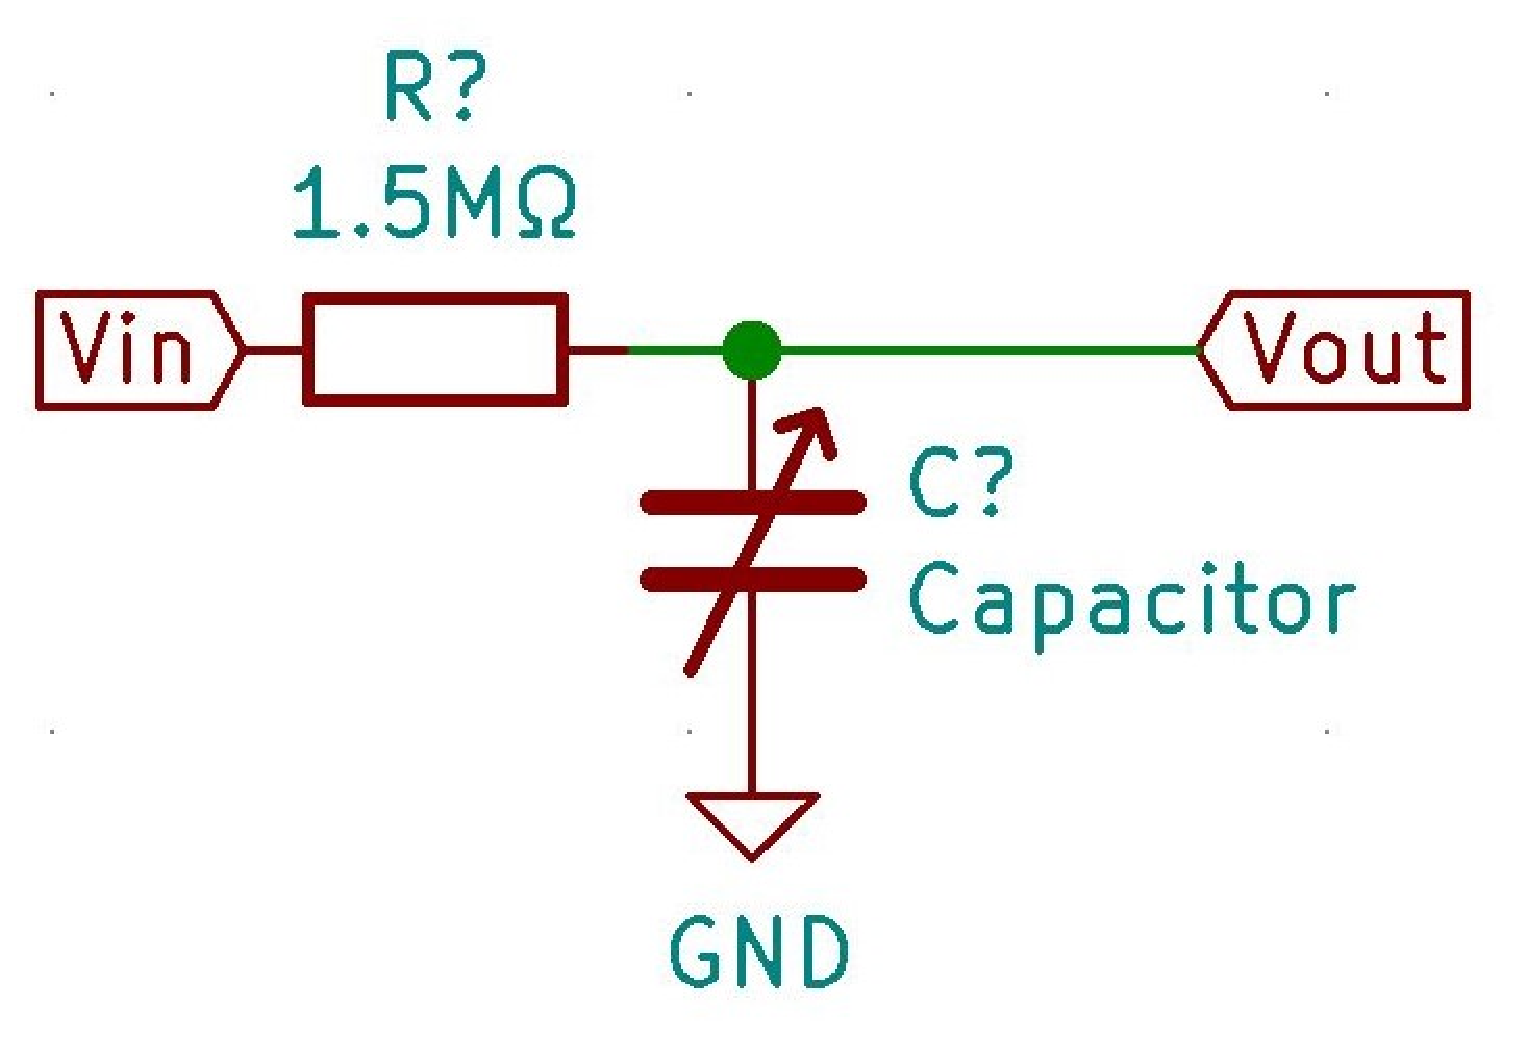
\includegraphics[width=0.5\columnwidth,clip]{./2_measurement/RC.eps}
  \caption{RC回路}
  \label{fig:RC}
 \end{center}
\end{figure}

\begin{figure}[h]
    \begin{center}
     \includegraphics[width=0.5\columnwidth,clip]{./2_measurement/oscilloscope.eps}
     \caption{fig:出力状態図}
     \label{オシロスコープ}
    \end{center}
\end{figure}

これらの計測に関して,1つのマイコンを用いて複数の伸縮センサの計測を行うと計測周期が低下し,
計測精度の低下が懸念された.これを踏まえ,1つのマイコンで計測を行う伸縮センサの数を2個とした.
一方で今回,足首を中心とした筋の伸縮の計測を行うため3チャンネル分の計測を行う必要がある.
故に,マイコン3枚分の計測システムを用意した.同期信号を用いて計測のデータ取得,同期を行った.
\begin{figure}[h]
 \begin{center}
  \includegraphics[width=0.5\columnwidth,clip]{./2_measurement/circuit.eps}
  \caption{計測時に実際に用いた基板}
  \label{fig:circuit}
 \end{center}
\end{figure}

\newpage

\subsection{足関節における筋肉}
%TODO:足首周りの動作関係のお話をする
%TODO:筋肉のお話もする
Fig.\ref{fig:legMuscle}において、脚部における筋肉状況を示す。これらの脚部筋肉のうち足関節の動作に
寄与している物はヒラメ筋、長腓骨筋、前脛骨筋、長母趾伸筋、長趾伸筋といったものが挙げられる。

従来のペダリングロボット、2足歩行ロボットの足関節部分では前脛骨筋、ヒラメ筋のみに注目し
それらの筋肉の再現を、空気圧人工筋を用いて行った。
今回製作する足関節ロボットでは実際の人間の動作の再現を行うため、従来のピッチ方向のみの動作を
想定した設計では目的を満たすことができない。そこで、従来注目していた、前脛骨筋、ヒラメ筋に
加えて、長腓骨筋も注目するようにした。また、従来のロボットでは足関節部分はピンジョイントを用いて、
動作方向の制限を行っていたが、今回はボールジョイントを用い、動作方向の制限をなくし、ロール・ピッチ・ヨー各方向に
自由度を持たせることができた。
\begin{figure}[h]
    \begin{center}
     \includegraphics[width=0.5\columnwidth,clip]{./2_measurement/legMuscle.eps}
     \caption{脚部における筋肉状況}
     \label{fig:legMuscle}
    \end{center}
\end{figure}

\newpage

\section{実験器具の製作}
\subsection{伸縮センサ製作}
\begin{enumerate}
    \item 3Dプリンターを用いて伸縮センサのサイズに合った型を用意する.
    \item 導電性布を型に合わせて鋏を用いて切る.
    \item 導電性布に錫めっき線を縫い通し,型の上に導電性布を置く.この際,錫めっき線が型の外に出てくるようにする.
    \item 上から硬化剤を混ぜたシリコン流し込み固まるまで数時間放置.
    \item シリコンが固まったら2枚目の導電性布に1枚目と同様に錫めっき線を通し硬化したシリコンの上に置く.
    \item その上から硬化剤を混ぜたシリコンを薄く塗り固まるまで放置.
    \item 最後のシリコンが硬化したら型から取り外し,錫めっき線に銅線接続し,コネクタをつけて完成.
\end{enumerate}
\subsection{足関節ロボット製作}

先述のとおり、以前製作されたペダリングロボット、2足歩行ロボットの経験をもとに足関節ロボットの製作を行った。
以下に足関節ロボットの製作過程を示す。
%TODO:使用した人体模型の種類の記述を行う。

今回、足関節ロボットの骨格としてFig.\ref{fig:bodyBone}人体模型を用いた。本模型から必要となる、膝より下の部分を取り外した。
取り外した結果、Fig.\ref{fig:legBone}の様になった。
\begin{figure}[h]
    \begin{center}
     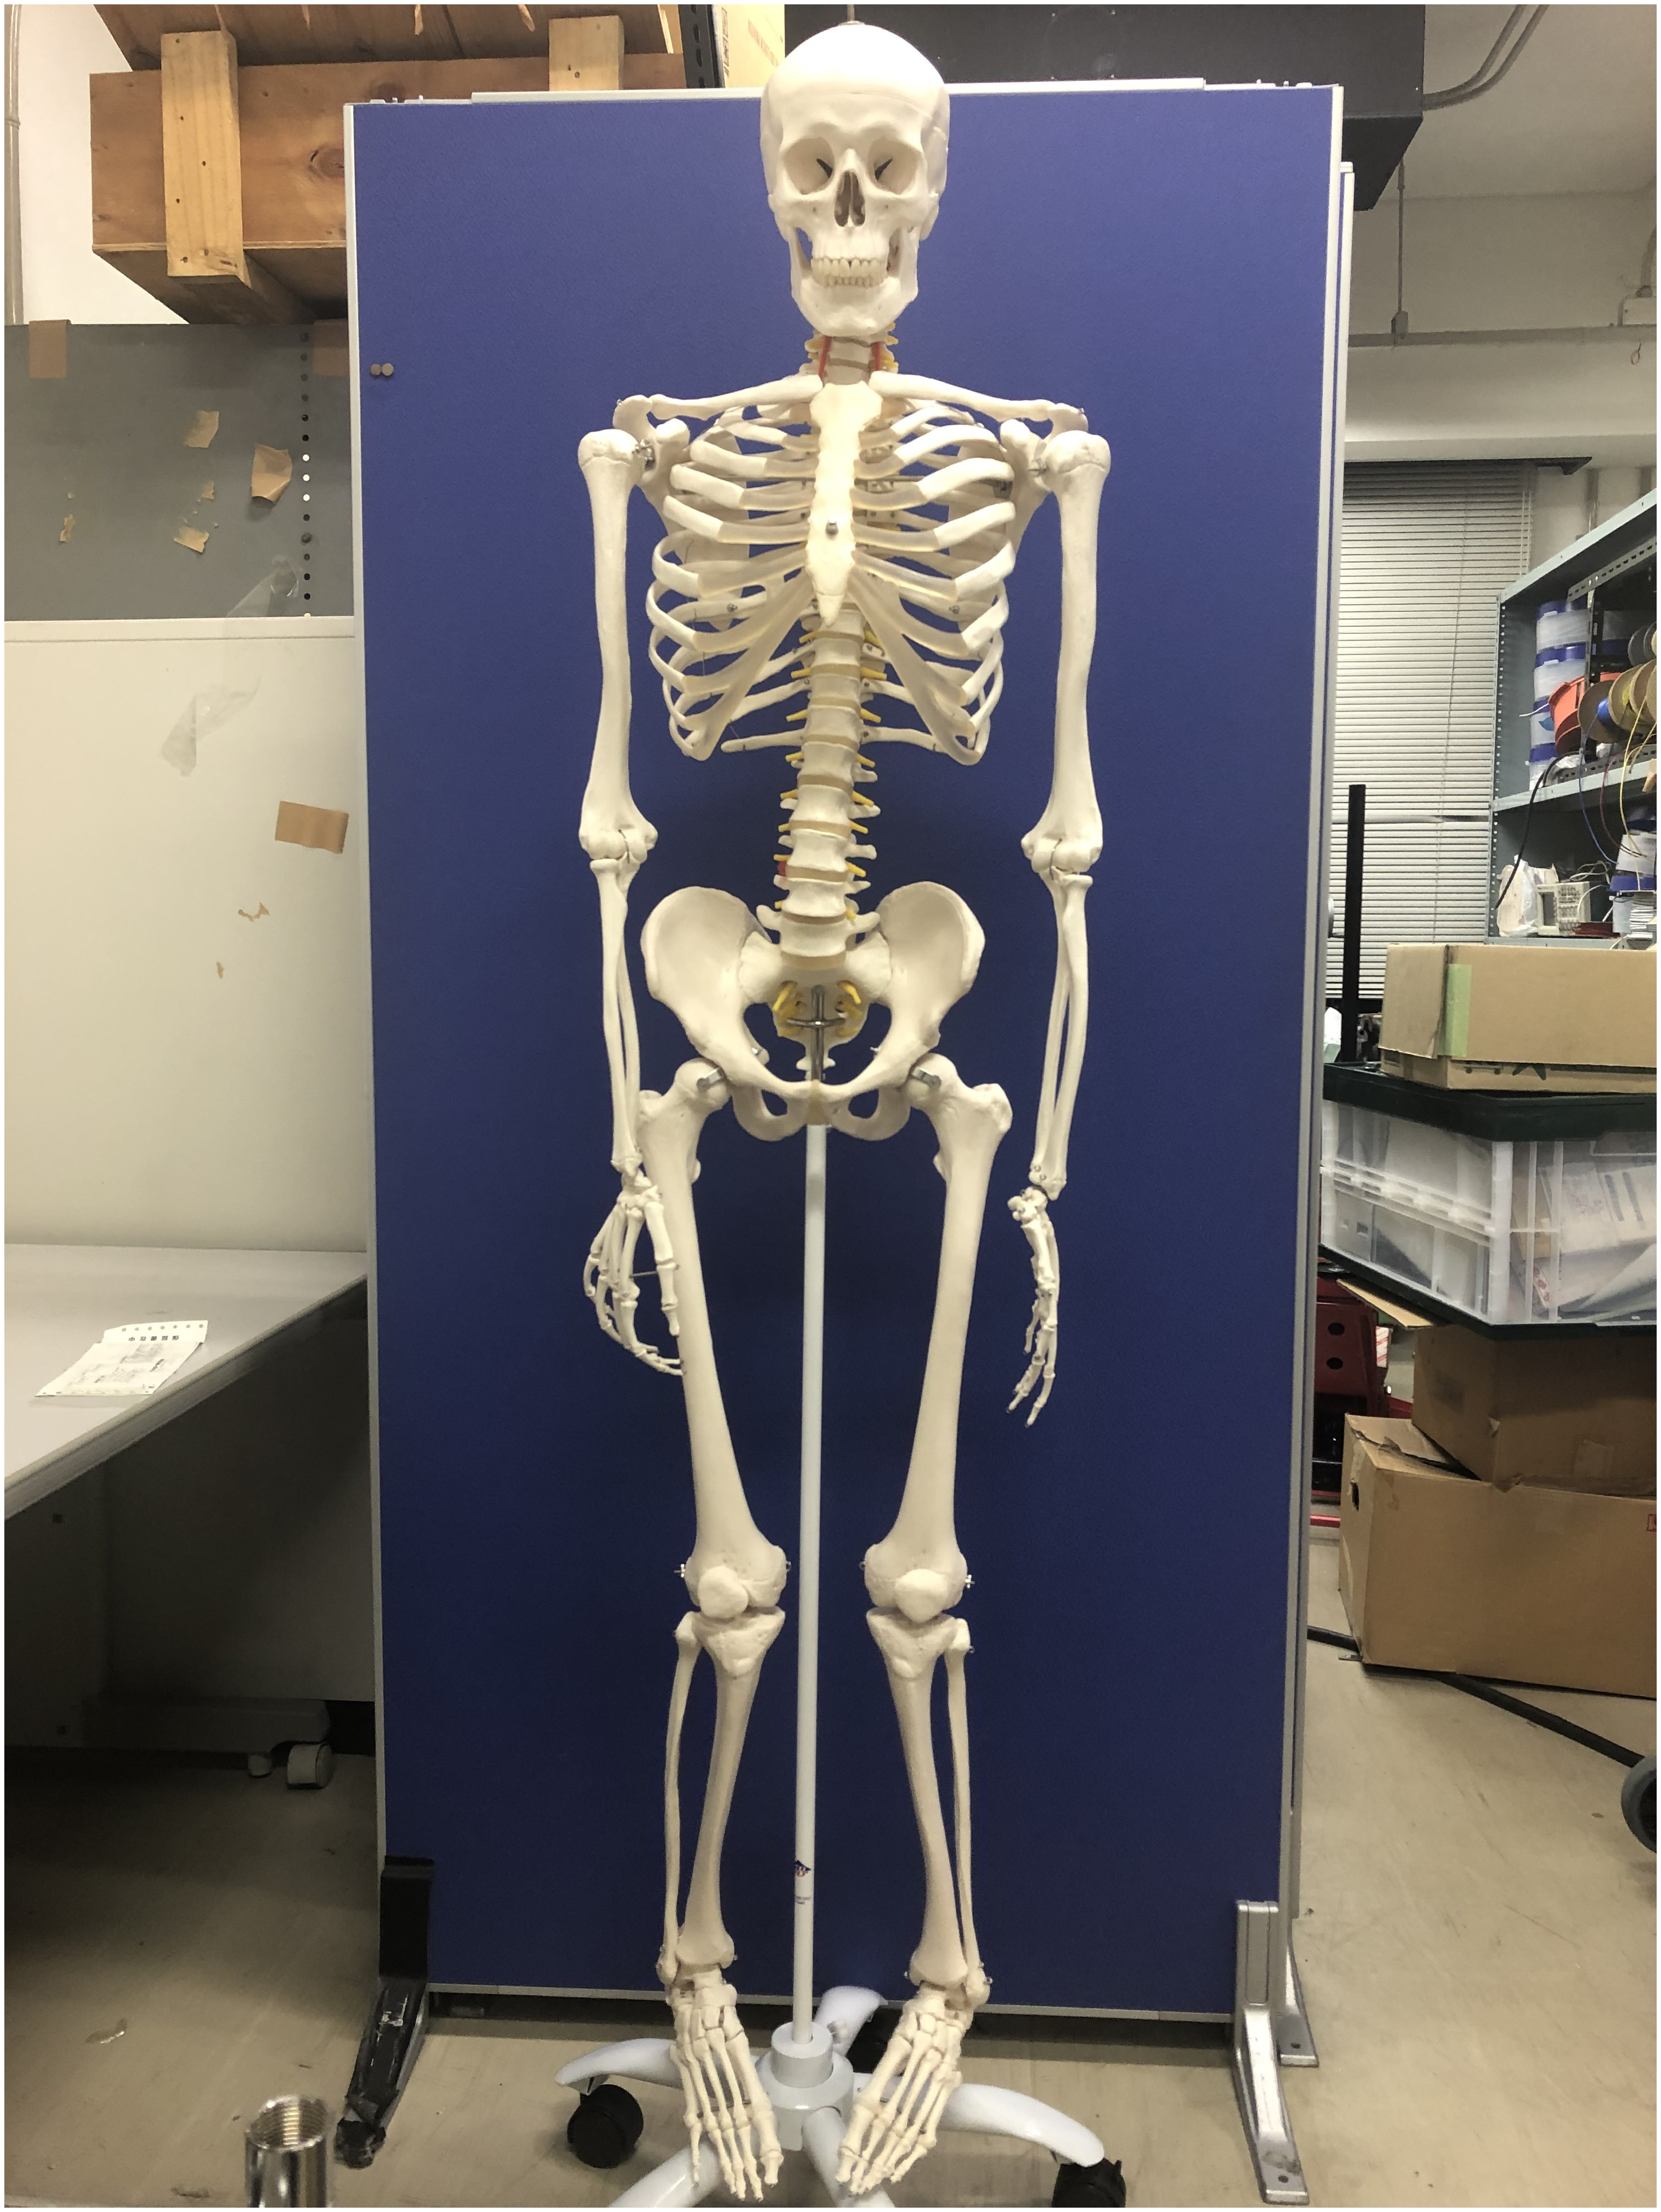
\includegraphics[width=0.4\columnwidth,clip]{./2_measurement/bodyBone.eps}
     \caption{人体模型骨格(全身)}
     \label{fig:bodyBone}
    \end{center}
    \begin{center}
     \includegraphics[width=0.6\columnwidth,clip]{./2_measurement/legBone.eps}
     \caption{人体模型骨格(脚部)}
     \label{fig:legBone}
    \end{center}
\end{figure}
\newpage
以前製作されたペダリングロボット、2足歩行ロボットでは関節部分にピンジョイントを用いていたが、今回製作する足関節ロボットでは、
自由度を向上させることを一つの目的としているので、膝部分にピンジョイント、足首部分にボールジョイントを用いた。

まず初めに前脛骨筋の両端を彫刻刀やバンドソーを用いて平面を作成した。続いてそこに、ボルト/ナットを用いてボールジョイント、ピンジョイントの軸受けの
固定を行った。そして、人間の筋付着位置に合わせて空気圧人工筋を接続するため、リングボルトを設置した。その結果、下記のFig.\ref{fig:legJoint}の様になった。

\begin{figure}[h]
    \begin{center}
     \includegraphics[width=0.6\columnwidth,clip]{./2_measurement/legJoint.eps}
     \caption{ジョイント、リングボルト接地状態(脚部)}
     \label{fig:legJoint}
    \end{center}
\end{figure}
次に重心位置を人間のものと合わせ、重量を成人男性の1/2にする作業を行った。
人体模型の骨は樹脂でできているため軽量であるので、鉛シートを巻き調整を行った。
重心位置の確認には紐で巻いて垂らし、その鉛直線が交わるところで求めた。
重量、重心位置の調整を行った結果、Fig.\ref{fig:legPb}の様になった。

\begin{figure}[h]
    \begin{center}
     \includegraphics[width=0.6\columnwidth,clip]{./2_measurement/legPb.eps}
     \caption{鉛シートを巻いた結果}
     \label{fig:legPb}
    \end{center}
\end{figure}
\newpage
続いて、足の製作を行った。前脛骨筋と同様に、人間の筋付着位置に合わせて空気圧人工筋の
接続をするリングボルトの設置をした。また、補強用として足の裏部分にアルミ板を固定した。
そして、ボールジョイント接続部分に穴をあけタップドリルを用いてねじ溝を掘った。

\begin{figure}[h]
    \begin{center}
     \includegraphics[width=0.6\columnwidth,clip]{./2_measurement/foot.eps}
     \caption{リングボルト設置結果(足上面)}
     \label{fig:foot}
    \end{center}
    \begin{center}
     \includegraphics[width=0.6\columnwidth,clip]{./2_measurement/footside.eps}
     \caption{リングボルト設置結果(足側面)}
     \label{fig:footside}
    \end{center}
\end{figure}

その後、指先と踵の間を丁番を用いて接続し、ピッチ方向に自由度を持たせた。
なお、空気圧人工筋などの能動的なアクチュエータは用いず、接地時に可動する受動的なものとして用いる様にした。
そして、その足にシリコン材を用いて肉付けを行い、重量、重心位置の調整をおこなった。
この時、脛骨と同様に重心位置は成人男性、重量は成人男性の1/2となるように調整をおこなった。
なお、脛骨と異なり鉛シートを用いずシリコン材を用いたのは衝撃吸収と成型性のしやすさからその様にした。
\newpage
\begin{figure}[h]
    \begin{center}
     \includegraphics[width=0.6\columnwidth,clip]{./2_measurement/siliconfoot.eps}
     \caption{シリコン材,丁番設置結果(足上面)}
     \label{fig:foot2}
    \end{center}
    \begin{center}
     \includegraphics[width=0.6\columnwidth,clip]{./2_measurement/siliconfootside.eps}
     \caption{シリコン材,丁番設置結果(足側面)}
     \label{fig:footside2}
    \end{center}
\end{figure}

続いて、脛骨と足部をボールジョイントのねじを用いて接続した。そして、人間の前脛骨筋、長腓骨筋、ヒラメ筋にあたる
空気圧人工筋3本を、それぞれワイヤーを用いてリングボルトと接続した。最後に、足部に靴を履かせて完成した。
完成したものは、Fig.\ref{fig:legPb}である。

\begin{figure}[h]
    \begin{center}
     \includegraphics[width=0.75\columnwidth,clip]{./2_measurement/fin.eps}
     \caption{完成した足関節ロボット}
     \label{fig:legPb}
    \end{center}
\end{figure}